% GunthaMeter project report: how the system works, step by step, and what is still pending.
% Compile: pdflatex main.tex  (twice, for the table of contents).  See README.md.
\documentclass[11pt,a4paper]{article}

\usepackage[T1]{fontenc}
\usepackage[utf8]{inputenc}
\usepackage{lmodern}
\usepackage{microtype}
\usepackage[margin=2.2cm]{geometry}
\usepackage{amsmath,amssymb}
\usepackage{booktabs}
\usepackage{tabularx}
\usepackage{longtable}
\usepackage{array}
\usepackage[table]{xcolor}
\usepackage{enumitem}
\usepackage{fancyhdr}
\usepackage{caption}
\usepackage{tikz}
\usetikzlibrary{arrows.meta,positioning,shapes.geometric,fit,calc,backgrounds}
\usepackage[hidelinks]{hyperref}

\definecolor{gmblue}{HTML}{0B3D6E}
\definecolor{gmok}{HTML}{1E7B34}
\definecolor{gmwarn}{HTML}{B35C00}
\definecolor{gmbad}{HTML}{A32020}
\definecolor{gmgrey}{HTML}{5A5F66}
\definecolor{gmlight}{HTML}{EEF3F8}

\newcommand{\done}{\textcolor{gmok}{\textbf{Done}}}
\newcommand{\partly}{\textcolor{gmwarn}{\textbf{Partly}}}
\newcommand{\pending}{\textcolor{gmbad}{\textbf{Pending}}}
\newcommand{\code}[1]{\texttt{\small #1}}
\newcommand{\INR}{INR~}
% timeline bar: {start week}{end week}{row}{label}{colour}
\newcommand{\gbar}[5]{\fill[#5] (#1,-#3+0.32) rectangle (#2,-#3-0.32);
  \node[anchor=east,font=\scriptsize] at (-0.3,-#3) {#4};}

\setlist{itemsep=2pt,topsep=4pt}
\setlength{\parskip}{4pt}
\setlength{\parindent}{0pt}
\setlength{\emergencystretch}{3em}
\renewcommand{\arraystretch}{1.18}

\pagestyle{fancy}
\fancyhf{}
\lhead{\small GunthaMeter --- Potholes, Fixed for Good}
\rhead{\small Project report, 14 November 2026}
\cfoot{\small \thepage}

\tikzset{
  box/.style={draw=gmblue, rounded corners=3pt, fill=gmlight, align=center, font=\small, inner sep=5pt,
              minimum height=9mm},
  gstep/.style={draw=gmblue, rounded corners=3pt, fill=white, align=center, font=\footnotesize, inner sep=4pt,
               text width=27mm, minimum height=11mm},
  st/.style={draw=gmblue, rounded corners=6pt, fill=gmlight, font=\scriptsize\ttfamily, inner sep=3pt,
             minimum height=6mm},
  arr/.style={-{Stealth[length=2.2mm]}, thick, gmblue},
  darr/.style={-{Stealth[length=2mm]}, gmgrey, dashed},
}

\begin{document}

% ------------------------------------------------------------------------------------------------- title
\begin{titlepage}
  \centering
  \vspace*{2.5cm}
  {\Huge\bfseries\color{gmblue} GunthaMeter\par}
  \vspace{4mm}
  {\Large Potholes, Fixed for Good\par}
  \vspace{10mm}
  {\large Bus-camera pothole detection $\rightarrow$ metric depth, area and volume with uncertainty
   $\rightarrow$ IRC:82 severity and priority $\rightarrow$ IRC:116 / SP:100 repair plan $\rightarrow$
   work orders, SLA escalation, bus-verified repair and defect-liability tracking\par}
  \vspace{14mm}
  {\Large\bfseries Project report: how the system works, step by step, and what is still pending\par}
  \vspace{12mm}
  {\large Telangana R\&B / Municipal Administration challenge\par}
  \vspace{4mm}
  {\large Status as of 14 November 2026\par}
  \vfill
  \begin{minipage}{0.86\textwidth}\small
  \textbf{How to read this report.} Section~\ref{sec:summary} gives the status in one page.
  Sections~\ref{sec:problem}--\ref{sec:steps} explain how the system works, one step at a time, in the order a
  pothole travels through it. Sections~\ref{sec:demo}--\ref{sec:evidence} show what has been demonstrated and
  measured. Sections~\ref{sec:status}--\ref{sec:pending} list what is finished and what is still pending, with
  effort estimates. Every number in this report is copied from the project's own artefacts
  (\code{reports/REPORT.md}, \code{reports/demo\_summary.json}, \code{docs/DECISIONS.md}); time and cost figures
  for the future are \emph{estimates} and are labelled as such.
  \end{minipage}
\end{titlepage}

\tableofcontents
\newpage

% ================================================================================================ 1
\section{Status at a glance}\label{sec:summary}

\textbf{The software is complete and verified on the development laptop.} All thirteen work packages of the
build plan (WP0--WP12) are implemented: the measurement core, the geo services, the database and API, the
processing workers, the operations services (work orders, SLA, verification, DLP), the web application, the bus
simulator, the validation scripts, the documentation and the one-command demo.

\textbf{What is \emph{not} finished is not code.} It is model training on a stronger GPU, a real-camera accuracy
session, certified camera calibration, building the Android app with the Android SDK, licence decisions, and a
field pilot on buses.

\begin{center}
\begin{tabularx}{\textwidth}{@{}l X r@{}}
\toprule
\textbf{Check} & \textbf{What it shows} & \textbf{Result}\\
\midrule
Python test suite & 276 automated tests (unit, API, workers, geo, end-to-end) & \textcolor{gmok}{276 passed}\\
Web application & unit tests, production build, offline smoke checks, browser tests & \textcolor{gmok}{38 / build OK / 15 / 3 passed}\\
Code style (ruff) & whole repository & \textcolor{gmok}{clean}\\
Measurement geometry & 16 synthetic road scenes with exact truth & \textcolor{gmok}{16/16, volume error $\le$ 2.9\,\%}\\
Uncertainty ($\sigma$) calibration & 200 noisy trials, truth inside $\pm2\sigma$ & \textcolor{gmok}{coverage 1.00 (target $\ge$ 0.90)}\\
Full demo & 3 simulated buses, 3 routes, 2 days, real Hyderabad roads & \textcolor{gmok}{4/4 acceptance checks, 732 s}\\
Detector accuracy & box mAP50 on the RDD-India test split (target $\ge$ 0.70) & \textcolor{gmbad}{0.0885 (no trained model yet)}\\
Real-camera depth accuracy & staged foam-board targets with a calibrated camera & \textcolor{gmbad}{not done yet}\\
\bottomrule
\end{tabularx}
\end{center}

\textbf{Estimated time to a validated pilot} (one to two developers; estimate, not a commitment): about
\textbf{1--2 weeks} for a trained model on an RTX-class GPU, \textbf{3--4 months} until the system is ready to
go on real buses, and about \textbf{6 months} including a 12-week pilot through a monsoon
(Section~\ref{sec:pending}).

% ================================================================================================ 2
\section{The problem}\label{sec:problem}

Potholes on city roads are reported late, measured by eye, repaired without proof, and often come back within
months. Four gaps cause most of this:
\begin{enumerate}
  \item \textbf{Finding them.} Surveys are occasional and manual; complaints arrive after the damage.
  \item \textbf{Measuring them.} Material and money are estimated by eye (``a few bags''), so neither the plan nor the
        bill can be checked.
  \item \textbf{Proving the repair.} A contractor's ``done'' photo is the only evidence that a repair happened and
        lasted.
  \item \textbf{Accountability.} When a repaired pothole reappears inside the contractor's defect-liability period
        (DLP), nobody notices in time to claim a free rework.
\end{enumerate}

\textbf{The idea.} TGSRTC buses already drive every arterial road many times a day. A camera behind the
windscreen turns every trip into a free survey. GunthaMeter closes the loop:
\emph{find $\rightarrow$ measure $\rightarrow$ prioritise $\rightarrow$ plan $\rightarrow$ repair $\rightarrow$ prove
the repair with later bus passes $\rightarrow$ catch the comeback}. It follows Indian standards throughout
(IRC:82-2015 for severity, IRC:116-2014 and IRC:SP:100-2014 for cold-mix repair) and uses Indian data only.

Three rules run through the whole system:
\begin{itemize}
  \item every measurement carries an uncertainty $\sigma$, the method used, and a quality score;
  \item cold-mix bags are always given as a low--high range, never as an ``exact'' number;
  \item demo calibrations are marked \code{certified=false} and are never used for billing.
\end{itemize}

% ================================================================================================ 3
\section{System architecture}\label{sec:arch}

\begin{figure}[h]
\centering
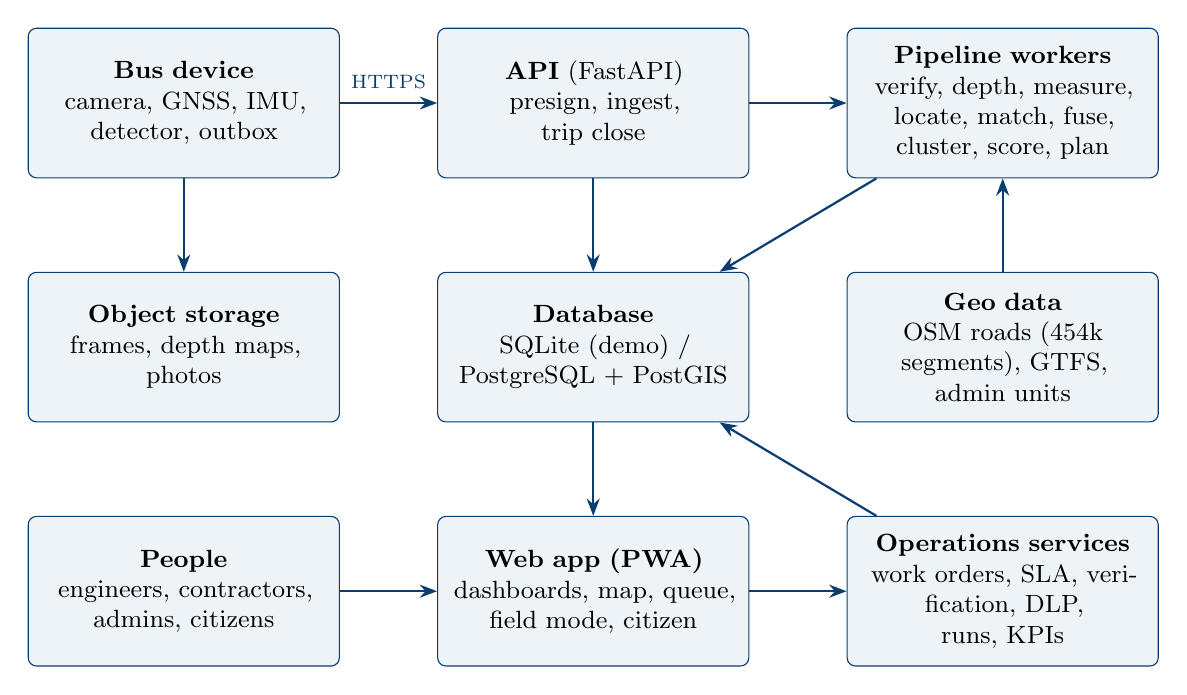
\begin{tikzpicture}[every node/.style={box, text width=36mm, minimum height=19mm}]
  % explicit 3 x 3 grid: columns 0 / 5.2 / 10.4 cm, rows 0 / -3.1 / -6.2 cm
  \node (bus)   at (0,0)       {\textbf{Bus device}\\camera, GNSS, IMU,\\detector, outbox};
  \node (api)   at (5.2,0)     {\textbf{API} (FastAPI)\\presign, ingest,\\trip close};
  \node (pipe)  at (10.4,0)    {\textbf{Pipeline workers}\\verify, depth, measure,\\locate, match, fuse,\\cluster, score, plan};
  \node (store) at (0,-3.1)    {\textbf{Object storage}\\frames, depth maps,\\photos};
  \node (db)    at (5.2,-3.1)  {\textbf{Database}\\SQLite (demo) /\\PostgreSQL + PostGIS};
  \node (geo)   at (10.4,-3.1) {\textbf{Geo data}\\OSM roads (454k\\segments), GTFS,\\admin units};
  \node (cit)   at (0,-6.2)    {\textbf{People}\\engineers, contractors,\\admins, citizens};
  \node (web)   at (5.2,-6.2)  {\textbf{Web app (PWA)}\\dashboards, map, queue,\\field mode, citizen};
  \node (ops)   at (10.4,-6.2) {\textbf{Operations services}\\work orders, SLA, veri-\\fication, DLP, runs, KPIs};
  \draw[arr] (bus) -- node[above, draw=none, fill=none, text width=, minimum height=0pt, font=\scriptsize]{HTTPS} (api);
  \draw[arr] (api) -- (pipe);
  \draw[arr] (bus) -- (store);
  \draw[arr] (api) -- (db);
  \draw[arr] (pipe) -- (db);
  \draw[arr] (geo) -- (pipe);
  \draw[arr] (ops) -- (db);
  \draw[arr] (db) -- (web);
  \draw[arr] (cit) -- (web);
  \draw[arr] (web) -- (ops);
\end{tikzpicture}
\caption{Main components. In the demo everything runs on one laptop (SQLite, filesystem storage, pipeline inside the
API process); production uses PostgreSQL/PostGIS, S3-compatible storage and separate worker processes.}
\end{figure}

\begin{center}
\begin{tabularx}{\textwidth}{@{}>{\raggedright\arraybackslash}p{36mm} X@{}}
\toprule
\textbf{Folder} & \textbf{Role}\\
\midrule
\code{edge/} & bus side: simulator (\code{sim/}), wire protocol (\code{protocol.md}, \code{schema/}), Jetson runner, Android skeleton\\
\code{measure/} & depth backends, road-plane fit, cavity measurement, uncertainty, fusion, IRC severity\\
\code{geo/} & ground-point location, map-matching, clustering, bus-pass counting, jurisdiction\\
\code{priority/}, \code{repair/} & priority score and SLA hours; repair planner (bags, materials, labour, cost)\\
\code{server/} & API, database models, workers (pipeline stages, ops ticks), operations services\\
\code{ml/} & segmenter interface, training, evaluation, export, pseudo-labelling\\
\code{web/} & React progressive web app (Telugu first, also Hindi and English), offline field mode\\
\code{gis/}, \code{data/} & map layers (zones, circles, wards, CRMP packages); dataset download and build\\
\code{scripts/}, \code{docs/}, \code{reports/} & demo and validation scripts; method and operations documents; results\\
\bottomrule
\end{tabularx}
\end{center}

% ================================================================================================ 4
\section{How the system works, step by step}\label{sec:steps}

This section follows one pothole from the camera to the closed, verified repair. Figure~\ref{fig:flow} shows the
steps; each subsection explains one of them.

\begin{figure}[h]
\centering
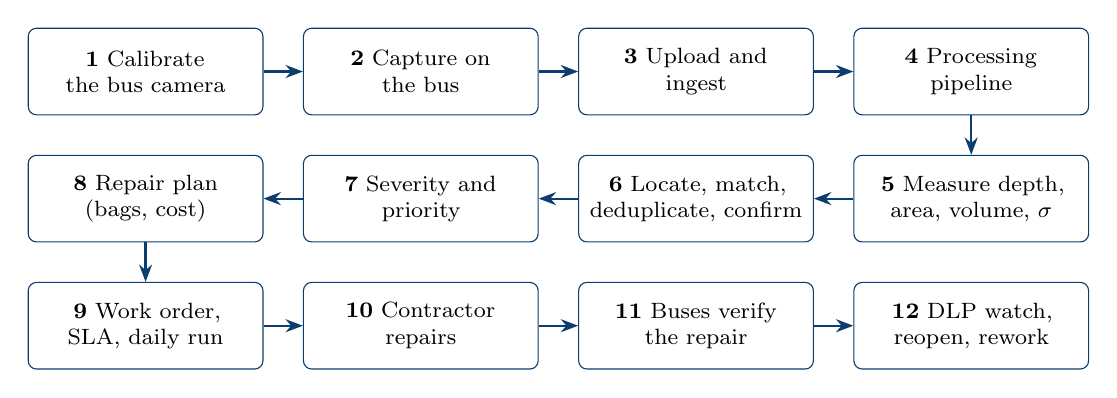
\begin{tikzpicture}[node distance=5mm and 5mm]
  \node[gstep] (s1) {\textbf{1} Calibrate\\the bus camera};
  \node[gstep, right=of s1] (s2) {\textbf{2} Capture on\\the bus};
  \node[gstep, right=of s2] (s3) {\textbf{3} Upload and\\ingest};
  \node[gstep, right=of s3] (s4) {\textbf{4} Processing\\pipeline};
  \node[gstep, below=of s4] (s5) {\textbf{5} Measure depth,\\area, volume, $\sigma$};
  \node[gstep, left=of s5] (s6) {\textbf{6} Locate, match,\\deduplicate, confirm};
  \node[gstep, left=of s6] (s7) {\textbf{7} Severity and\\priority};
  \node[gstep, left=of s7] (s8) {\textbf{8} Repair plan\\(bags, cost)};
  \node[gstep, below=of s8] (s9) {\textbf{9} Work order,\\SLA, daily run};
  \node[gstep, right=of s9] (s10) {\textbf{10} Contractor\\repairs};
  \node[gstep, right=of s10] (s11) {\textbf{11} Buses verify\\the repair};
  \node[gstep, right=of s11] (s12) {\textbf{12} DLP watch,\\reopen, rework};
  \draw[arr] (s1)--(s2); \draw[arr] (s2)--(s3); \draw[arr] (s3)--(s4); \draw[arr] (s4)--(s5);
  \draw[arr] (s5)--(s6); \draw[arr] (s6)--(s7); \draw[arr] (s7)--(s8); \draw[arr] (s8)--(s9);
  \draw[arr] (s9)--(s10); \draw[arr] (s10)--(s11); \draw[arr] (s11)--(s12);
\end{tikzpicture}
\caption{The twelve steps. Step 13 (dashboards, citizens, public reporting) reads from all of them.}
\label{fig:flow}
\end{figure}

% ------------------------------------------------------------------------------------------- step 1
\subsection{Step 1 --- Calibrate the bus camera}
Depth from a single camera is only metric if the system knows the camera's geometry. Each device gets a
\emph{calibration certificate} (\code{configs/cameras/*.json}):
\begin{itemize}
  \item \textbf{Intrinsics} (once per camera model): focal lengths $f_x, f_y$, principal point $c_x, c_y$ and lens
        distortion, from 20--25 photos of a $9\times6$ checkerboard. Accepted if the reprojection error is below
        0.3 pixels.
  \item \textbf{Extrinsics} (every bus, about 10 minutes at the depot): the camera height $h_{\text{true}}$ measured
        with a tape ($\pm1$\,cm; about 2.2--2.5\,m on a bus), pitch, roll and yaw from four cones at 3/5/8/12\,m.
        Accepted if a painted $1\,\text{m}\times1\,\text{m}$ square at 5\,m is reconstructed within 5\,\%.
  \item \textbf{Drift checks} on every trip: if the camera height implied by the road plane drifts by more than
        5\,\% or the pitch by more than $3^\circ$, the server raises an alert and the bus is recalibrated.
\end{itemize}
A certificate becomes \code{certified=true} only when both acceptance tests pass, and billing-grade only after a
per-device truth fit on at least 20 inspector-measured potholes. The procedure is written up for depot staff in
\code{docs/CALIBRATION\_SOP.md} (Telugu and English).

% ------------------------------------------------------------------------------------------- step 2
\subsection{Step 2 --- Capture on the bus}
The device (an Android phone, a Jetson box, or the simulator) runs the same loop:
\begin{enumerate}
  \item \textbf{Keyframe trigger.} A frame is analysed every 4\,m of travel while the bus drives faster than
        5\,km/h (values from the signed edge configuration).
  \item \textbf{Detection.} An on-device segmenter (YOLO26n-seg) outputs, per pothole, its class, confidence,
        bounding box and outline polygon, plus a track id. At most 3 keyframes are kept per tracked pothole.
  \item \textbf{Privacy.} Faces and number plates are blurred on the device before anything is stored.
  \item \textbf{Observation.} One JSON record per keyframe with detections: device, trip, sequence number, time
        (IST), GNSS fix (position, accuracy, speed, heading), IMU summary and the frame key. Its
        \code{client\_uuid} is fixed at creation, so resending it is harmless.
  \item \textbf{IMU jolt.} When a wheel drops into a pothole, the vertical-acceleration spike produces a
        ``jolt'' observation. A jolt confirms that a pothole exists; it never sets the depth on its own.
  \item \textbf{Trip fixes.} A GNSS fix every second, with a \code{cam\_active} flag. These later prove that the
        bus passed a repaired spot with the camera on.
  \item \textbf{Outbox.} Everything waits in a durable queue until the server has acknowledged it.
\end{enumerate}

% ------------------------------------------------------------------------------------------- step 3
\subsection{Step 3 --- Upload and ingest}
Uploads happen over LTE or, by default for frames, over depot Wi-Fi. The order is fixed (\code{edge/protocol.md}):
\begin{enumerate}
  \item \code{POST /v1/edge/presign} returns upload URLs; frames are uploaded with \code{PUT};
  \item \code{POST /v1/ingest/observations} (up to 200 per batch, idempotent by \code{client\_uuid});
  \item \code{POST /v1/ingest/trip-fixes} (up to 600 per batch);
  \item \code{POST /v1/ingest/trip-close}, which builds the trip geometry and runs the trip-close hooks
        (bus-pass counting and repair verification, Step 11).
\end{enumerate}
Every call can be retried safely after a network error; the server removes duplicates.

% ------------------------------------------------------------------------------------------- step 4
\subsection{Step 4 --- The processing pipeline}
Each observation runs through nine stages, inside the API in the demo or in separate worker processes in
production:
\begin{center}
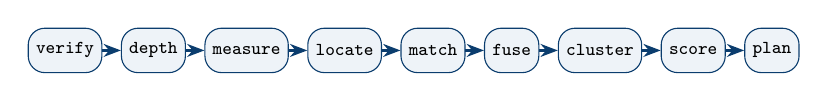
\begin{tikzpicture}[node distance=2.5mm, scale=0.94, transform shape]
  \foreach \n/\t [count=\i] in {v/verify, d/depth, m/measure, l/locate, mm/match, f/fuse, c/cluster, s/score, p/plan}{
    \ifnum\i=1 \node[st] (\n) {\t}; \else \node[st, right=of \last] (\n) {\t}; \fi
    \xdef\last{\n}
  }
  \foreach \a/\b in {v/d, d/m, m/l, l/mm, mm/f, f/c, c/s, s/p}{ \draw[arr] (\a)--(\b); }
\end{tikzpicture}
\end{center}
\textbf{verify}: an optional second detector checks each detection. \textbf{depth}: a metric depth model
(Depth-Anything-V2 Metric Outdoor by default) estimates the distance of every pixel. \textbf{measure}: depth,
area and volume with $\sigma$ (Step 5). \textbf{locate} and \textbf{match}: the pothole's ground position and road
segment (Step 6). \textbf{fuse}: frames are combined into one measurement per bus pass. \textbf{cluster}: the
observation joins an existing pothole or creates a new one. \textbf{score}: severity and priority (Step 7).
\textbf{plan}: repair plan (Step 8). A failing stage is recorded as an error; no stage quietly falls back to a
cruder method.

% ------------------------------------------------------------------------------------------- step 5
\subsection{Step 5 --- Measure depth, area and volume (with \texorpdfstring{$\sigma$}{sigma})}
Details: \code{docs/DEPTH\_METHOD.md}. In short:
\begin{enumerate}
  \item \textbf{Back-projection.} For pixel $(u,v)$ with depth $Z$: $X=(u-c_x)Z/f_x$, $Y=(v-c_y)Z/f_y$.
  \item \textbf{Road plane.} RANSAC fits a plane $n\cdot p + d = 0$ to road pixels (lower 65\,\% of the image, potholes
        masked out, 2.5--14\,m range; 15\,mm inlier band). The frame is rejected if fewer than half the points fit,
        the residual exceeds 25\,mm, or the plane's pitch differs from the calibration by more than $4^\circ$.
  \item \textbf{Scale lock.} The plane's distance from the camera, $\hat h=|d|$, is the height the depth model
        believes the camera is at. Multiplying every depth by $s=h_{\text{true}}/\hat h$ (allowed range 0.5--2.0)
        removes the 5--30\,\% absolute-scale error of monocular depth models with one tape measurement.
  \item \textbf{Local road surface.} Around each pothole (ring 0.3--1.2\,m), a quadratic surface
        $y_s=a+bx+cz+dx^2+ez^2+fxz$ follows the road's camber and ruts.
  \item \textbf{Cavity depth and footprint.} For each mask pixel $i$: depth below the road
        $\delta_i=\max(0,\,y_s(x_i,z_i)-y_i)$ and ground footprint $a_i=(Z_i/f_x)(Z_i/f_y)/\cos\theta_i$.
  \item \textbf{Metrics.}
        \[ A=\sum_i a_i,\qquad V=\sum_i \delta_i a_i,\qquad d_{p95}=\text{95th percentile of }\delta_i
           \text{ weighted by } a_i, \]
        plus length and width from the minimum-area rectangle. $d_{p95}$ is the design depth.
  \item \textbf{Uncertainty.} Depth noise grows with distance: $\sigma_{Z,i}=k Z_i^2$ with
        $k=4\times10^{-4}\,\text{m}^{-1}$ until a per-device fit exists. It combines with the surface-fit residual and
        the scale uncertainty into $\sigma_{\delta,i}$, and from there into $\sigma$ for $d_{p95}$, $A$ and
        $V$ (volume errors are treated as fully correlated, which is conservative).
  \item \textbf{Quality} $q\in[0,1]$: product of gates for range (best at 3--7\,m, zero beyond 12\,m), blur,
        lighting, mask confidence, plane fit and mask size.
  \item \textbf{Fusion.} Frames with $q<0.2$ and outliers beyond $3\sigma$ are dropped; the rest are averaged with
        weights $q_j/\sigma_j^2$, first into one measurement per pass, then into the pothole.
  \item \textbf{Water.} A water-filled pothole gets \emph{unknown} depth (never the water surface), a severity lower
        bound from its width, and a re-measure 48\,h after rain.
\end{enumerate}

% ------------------------------------------------------------------------------------------- step 6
\subsection{Step 6 --- Locate, match to a road, deduplicate, confirm}
\begin{itemize}
  \item \textbf{Ground point.} The GNSS fix, advanced by the receiver latency and offset by the pothole's measured
        forward and lateral distance along the bus heading. Position uncertainty
        $\sigma_{\text{pos}}=\sqrt{\text{gps\_accuracy}^2+(0.05D)^2}$.
  \item \textbf{Map-matching.} The nearest OpenStreetMap road segments within 25\,m whose direction agrees with
        the bus heading (within $\pm45^\circ$); output: road (\code{way\_id}), direction, chainage and lane band.
  \item \textbf{Clustering.} Observations on the same road and direction within about 6\,m (or
        $2.5\,\sigma$ for noisy fixes across trips) are the same pothole.
  \item \textbf{Confirmation.} A pothole starts as a \code{candidate} and becomes \code{confirmed} after
        $\ge2$ passes from $\ge2$ different trips, or one pass plus a citizen report within 25\,m, or one pass plus
        an IMU jolt with quality $\ge0.6$.
  \item \textbf{Owner.} The road segment gives the owning agency and CRMP contract. If no owner is known, the
        pothole goes to the \emph{jurisdiction queue} for an administrator, and is provisionally shown to the
        agency of the admin unit it lies in, so that nothing is silently dropped.
\end{itemize}

% ------------------------------------------------------------------------------------------- step 7
\subsection{Step 7 --- Severity and priority}
\textbf{Severity (IRC:82-2015):} small ($d_{p95}\le25$\,mm and width $\le200$\,mm), medium ($\le50$\,mm and
$\le500$\,mm), otherwise large.

\textbf{Priority} (0--100), editable per agency and versioned:
\[ P = 100\cdot\operatorname{clip}\big(0.30\,S+0.25\,E+0.20\,V+0.15\,T+0.10\,M,\ 0,\ 1\big) \]
\begin{tabularx}{\textwidth}{@{}l X@{}}
\toprule
\textbf{Term} & \textbf{Meaning}\\
\midrule
$S$ severity & large 1.0, medium 0.6, small 0.3; +0.2 in a wheel path or near a junction; +0.1 if an IMU jolt confirmed it\\
$E$ exposure & road class (trunk/primary 1.0 \ldots\ service 0.2) and bus passes per day\\
$V$ vulnerability & schools, hospitals, bus stops, metro stations, markets within 200\,m; unlit roads\\
$T$ age & hours since confirmation relative to the SLA; +0.3 if breached; citizen complaints\\
$M$ monsoon & monsoon window, recent heavy rain, waterlogging hotspot, water-filled\\
\bottomrule
\end{tabularx}

% ------------------------------------------------------------------------------------------- step 8
\subsection{Step 8 --- Repair plan}
Following IRC:82 (cut to sound material), IRC:116-2014 (ready-made cold mix, at least 50\,mm) and IRC:SP:100-2014:
\begin{enumerate}
  \item square cut with a 0.125\,m margin: $A_{\text{cut}}=(L+0.25)(W+0.25)$;
  \item design depth $=\max(d_{p95}, 50\,\text{mm})$ rounded up to 5\,mm; deeper than 75\,mm becomes two layers;
  \item mix mass $M=A_{\text{cut}}\cdot d\cdot\rho\cdot(1+w)$ with $\rho=2200$\,kg/m$^3$ and 12\,\% wastage;
  \item bags $=\lceil M/25\,\text{kg}\rceil$ with a low--high range from $\sigma_M$; then emulsion, sand, labour hours
        and cost from the agency's rate card.
\end{enumerate}
\textbf{Worked example} (a unit test): a $0.50\times0.40$\,m pothole, $d_{p95}=60$\,mm: cut $0.4875$\,m$^2$, 72.1\,kg of
mix, \textbf{3 bags (range 3--4)}, about \INR1,406 against the reported baseline of \INR7,396 per pothole. The method
selector can also choose emulsion mix, a jet patcher (clusters), infrared or hot mix.

% ------------------------------------------------------------------------------------------- step 9
\subsection{Step 9 --- Work order, SLA and the daily repair run}
An engineer (or the planner) creates a \emph{work order} for one or more potholes. It is issued to the contractor of
the road's CRMP package (or to a contractor the engineer assigns). The SLA clock starts at issue: 24\,h on arterial
roads, 72\,h on other roads in the monsoon, 168\,h off-season or on R\&B roads.

\textbf{Escalation ladder} (checked every 5 minutes): 50\,\% of the SLA $\rightarrow$ Assistant Engineer;
breach $\rightarrow$ Deputy Executive Engineer; +24\,h $\rightarrow$ Executive Engineer; +72\,h $\rightarrow$ Zonal
Commissioner. Each step is stored and audited.

\textbf{Daily run} (06:00 IST, per circle): issued work orders are ordered into a nearest-neighbour route, capped by
crew hours, and printed as an \emph{indent} (bags, emulsion, sand, crew hours, cost).

% ------------------------------------------------------------------------------------------- step 10
\subsection{Step 10 --- The contractor repairs}
In the field mode of the web app (which works offline): \code{acknowledged} $\rightarrow$ \emph{before} photo
$\rightarrow$ \code{in\_progress} (bag lot number) $\rightarrow$ \emph{after} photo and bags used $\rightarrow$
\code{repaired\_claimed}. Photos queue offline and sync when the network returns. A contractor can only act on their
own work orders and can never verify their own repair. Every transition is written to the audit log.

% ------------------------------------------------------------------------------------------- step 11
\subsection{Step 11 --- Buses verify the repair}
A repair claim is not a repair. After the claim, every bus trip that passes the spot (same road, direction and
lane band, camera on) without detecting the pothole counts as a \emph{clean pass}. The work order becomes
\code{verified\_closed} after \textbf{$\ge3$ clean passes from $\ge2$ different trips within 14 days}, and after a
10\,\% random engineer QC sample (when drawn) is passed. Only \code{verified\_closed} work orders are eligible for
invoicing and the Measurement Book.

% ------------------------------------------------------------------------------------------- step 12
\subsection{Step 12 --- DLP watch, reopen and rework}
A verified repair stays under watch. If a bus detects the pothole again inside the defect-liability period (6
months for a patch by default; 5 years for a CRMP package), the pothole is \code{reopened}, a \code{dlp\_event} is
recorded with an \emph{evidence package} (before/after photos, re-detection frames, measurements, pass log), and a
zero-pay rework work order is drafted for the same contractor. It is evidence for the engineer, not an automatic
penalty. Contractor scorecards show SLA compliance, verified closures, DLP events and the reopen rate.

\begin{figure}[h]
\centering
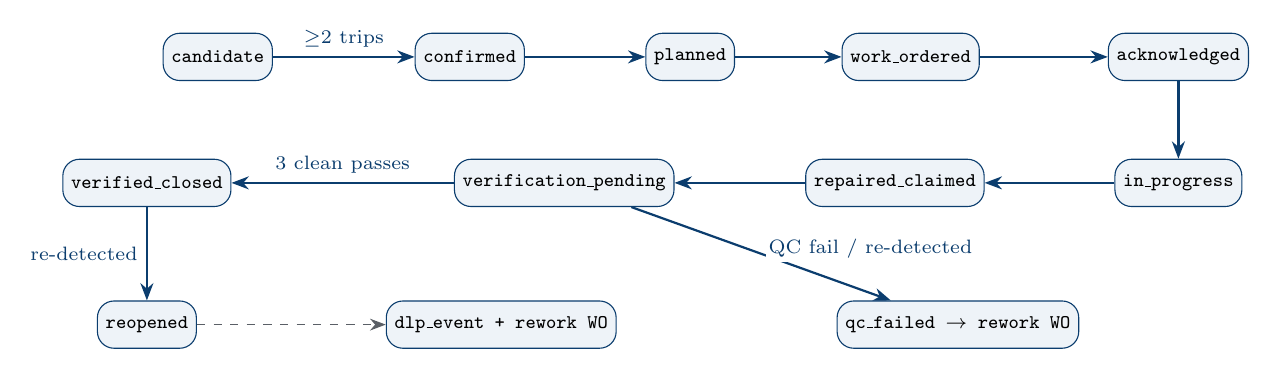
\begin{tikzpicture}[lbl/.style={font=\scriptsize, fill=white, inner sep=1pt}]
  % row 1 (left to right), row 2 (right to left), row 3 (outcomes); x in cm
  \node[st] (c)  at (0,0)     {candidate};
  \node[st] (cf) at (3.2,0)   {confirmed};
  \node[st] (pl) at (6.0,0)   {planned};
  \node[st] (wo) at (8.8,0)   {work\_ordered};
  \node[st] (ak) at (12.2,0)  {acknowledged};
  \node[st] (ip) at (12.2,-1.6) {in\_progress};
  \node[st] (rc) at (8.6,-1.6)  {repaired\_claimed};
  \node[st] (vp) at (4.4,-1.6)  {verification\_pending};
  \node[st] (vc) at (-0.9,-1.6) {verified\_closed};
  \node[st] (ro) at (-0.9,-3.4) {reopened};
  \node[st] (dlp) at (3.6,-3.4) {dlp\_event + rework WO};
  \node[st] (qf) at (9.4,-3.4)  {qc\_failed $\rightarrow$ rework WO};
  \draw[arr] (c)--node[lbl, above=2pt]{$\geq$2 trips}(cf);
  \draw[arr] (cf)--(pl); \draw[arr] (pl)--(wo); \draw[arr] (wo)--(ak);
  \draw[arr] (ak)--(ip); \draw[arr] (ip)--(rc); \draw[arr] (rc)--(vp);
  \draw[arr] (vp)--node[lbl, above=2pt]{3 clean passes}(vc);
  \draw[arr] (vc)--node[lbl, left=2pt]{re-detected}(ro);
  \draw[darr] (ro)--(dlp);
  \draw[arr] (vp) -- node[lbl, right=6pt, pos=0.45]{QC fail / re-detected} (qf);
\end{tikzpicture}
\caption{Pothole life cycle (simplified; \code{rejected}, \code{archived} and \code{recurrence\_watch} omitted).}
\end{figure}

% ------------------------------------------------------------------------------------------- step 13
\subsection{Step 13 --- Dashboards, citizens and public reporting}
The web app (Telugu first, also Hindi and English) offers: a zonal dashboard with KPIs; a map coloured by severity
or priority; a pothole page with frames, mask, depth cross-section, measurement $\pm\sigma$ and the repair plan; the
priority queue; work orders; repair runs and indents; the offline field mode; contractor scorecards; an admin area
(priority weights, rate card, SLA, admin units, jurisdiction queue, audit log); a citizen page to report a pothole
and track it with a ticket; and a public ward league.

% ================================================================================================ 5
\section{The simulator and the end-to-end demo}\label{sec:demo}

Real buses are not yet equipped, so the whole loop is exercised with \emph{virtual buses}
(\code{edge/sim/}). They drive real TGSRTC GTFS route shapes over real OpenStreetMap Hyderabad roads, paste real
Indian pothole images (from labelled datasets) into keyframes at geometrically correct positions, add GNSS noise
and receiver latency, and speak the same protocol as a real device. \code{edge/sim/fleet.py} runs several buses
over several routes and days:
\begin{enumerate}
  \item \textbf{survey days}: 3 trips per route per day, 2 IMU jolts, 1 citizen report (in Telugu), and a stretch of
        road outside every admin circle (to exercise the jurisdiction queue);
  \item \textbf{repair day}: work orders are created and a contractor claims repairs through the API;
  \item \textbf{verification days}: repaired potholes are no longer seen, so passes are clean;
  \item \textbf{DLP check}: one verified repair is detected again.
\end{enumerate}
\code{scripts/demo.py} (\code{tasks.ps1 demo} / \code{make demo}) copies the seeded database, starts the API and web
app, runs the fleet, issues tomorrow's work orders and repair runs, and prints a summary.

\textbf{Important:} in the demo the depth of each frame is a synthetic road render (method \code{synthetic}),
because the real depth model takes 5--20\,s per frame on a laptop CPU. The demo proves the pipeline and the
operations loop, not measurement accuracy.

\begin{center}
\begin{tabularx}{\textwidth}{@{}X r r@{}}
\toprule
\textbf{Demo run of 14 Nov 2026} (3 buses; routes 10H, 218, 5K; 2 days; 21 trips) & \textbf{Result} & \textbf{Target}\\
\midrule
Potholes ever confirmed & 43 & $\ge30$\\
Repairs verified by bus passes & 2 potholes / 3 work orders & $\ge1$\\
Reopened inside DLP, with a zero-pay rework order & 1 & $\ge1$\\
Jurisdiction-queue items & 4 & $\ge1$\\
Fleet run time & 714\,s & $<15$\,min\\
Whole demo from a clean database copy & 732\,s & $<20$\,min\\
\midrule
Tomorrow's indent & \multicolumn{2}{r}{8 work orders, 49--60 bags (range), 3 circles}\\
30-day estimated repair cost vs baseline (2 zones) & \multicolumn{2}{r}{\INR63,922 vs \INR2,81,048}\\
\bottomrule
\end{tabularx}
\end{center}
Three work orders stayed \code{verification\_pending}; one of them by design (the 10\,\% QC sample waiting for an
engineer). A first full run before two simulator fixes reached only 2 of the 4 checks; both fixes are described in
\code{docs/DECISIONS.md}.

% ================================================================================================ 6
\section{Evidence: what has been measured}\label{sec:evidence}

\subsection{Measurement geometry (verified)}
Rendered roads with a cavity of known shape, at known camera height and pitch; the depth map is exact, so this
checks the geometry and the uncertainty formulas, not a depth model.

\begin{center}
\small
\begin{tabular}{@{}l r r r r r@{}}
\toprule
\textbf{Case} & \textbf{True L} & \textbf{Measured L} & \textbf{Err.} & \textbf{True p95} & \textbf{Meas. p95}\\
\midrule
car 1.4\,m, plane, cap 0.8\,m$\times$50\,mm @ 4\,m & 12.63 & $12.63\pm1.35$ & +0.0\,\% & 47.5 & 47.5\\
car 1.4\,m, plane, same cap @ 10\,m & 12.63 & $13.00\pm4.15$ & +2.9\,\% & 47.5 & 47.0\\
bus 2.4\,m, plane, same cap @ 5\,m & 12.63 & $12.63\pm2.77$ & +0.0\,\% & 47.5 & 47.5\\
bus 2.4\,m, crown, cap 1.0\,m$\times$70\,mm @ 8\,m & 27.72 & $27.69\pm6.77$ & $-0.1$\,\% & 66.8 & 66.7\\
car, plane, box 0.7\,m$\times$60\,mm @ 7\,m & 23.09 & $22.51\pm4.39$ & $-2.5$\,\% & 60.0 & 60.0\\
\bottomrule
\end{tabular}
\end{center}
All 16 cases pass (5 shown; full table in \code{reports/REPORT.md}): maximum volume error 2.9\,\%, maximum p95
error 0.6\,mm. In 200 noisy trials the truth lay inside $\pm2\sigma$ every time (coverage 1.00 for depth, volume,
area and width; target $\ge0.90$), so the reported $\sigma$ is conservative.

\subsection{Staged known-depth targets (protocol ready, real run pending)}
The procedure for foam-board ``potholes'' of 20/40/70\,mm filmed at 3--12\,m is scripted in
\code{scripts/staged\_pothole\_truth.py}. It has been \emph{rehearsed} on rendered targets: fused depth error
1.7\,mm, volume error 12.0\,\%, IRC class 100\,\% correct (targets: $\le10$\,mm, $\le25$\,\%, $\ge90$\,\%). This rehearsal
tests the scripts; it says nothing about a real camera. The real session is pending.

\subsection{Real Indian road images (chain runs; not measurements)}
The real depth model ran on 6 dataset images with an uncertified demo calibration. The true camera height and
angle of those photos are unknown, and the pipeline flagged this itself in every case (scale outside $[0.5,2]$ in
6/6, quality $<0.6$ in 6/6). This shows the safety gates working, not accuracy.

\subsection{Detector}
The starter (bootstrap) detector scores box mAP50 \textbf{0.0885} on the RDD-India test split (514 images, 1,038
potholes), far below the 0.70 target. The training code is finished; the training run itself is pending
(Section~\ref{sec:pending}).

% ================================================================================================ 7
\section{Status by work package}\label{sec:status}

\begin{longtable}{@{}p{0.29\textwidth} p{0.10\textwidth} p{0.55\textwidth}@{}}
\toprule
\textbf{Work package} & \textbf{State} & \textbf{Notes}\\
\midrule
\endhead
WP0 Scaffold and contracts & \done & frozen interfaces in \code{docs/CONTRACTS.md}\\
WP1 Data acquisition & \done & RDD2022 India, eYantra masks, BharatPotHole (licence unverified, excluded by default), OSM, GTFS\\
WP2 Measurement core & \done & synthetic 16/16, $\sigma$ coverage 1.00; real-camera accuracy pending\\
WP3 Training, export & \partly & all code done (segmenter, training, evaluation, export, pseudo-labels); \textbf{no trained model}\\
WP4 Database, API & \done & 50+ endpoints, role-based access, audit log\\
WP5 Geo services & \done & PostGIS map-matching SQL never run against a real PostGIS\\
WP6 Workers & \done & nine pipeline stages, ops ticks, job poller\\
WP7 Edge simulator & \done & fleet acceptance 4/4; Android skeleton not compiled (no SDK); Jetson runner is a stub\\
WP8 Ops, repair planner & \done & state machines, SLA ladder, verification, DLP, runs, KPIs, MB/invoice exports\\
WP9 Web app & \done & tests, build, offline smoke and browser tests pass; Lighthouse audit not run\\
WP10 GIS layers & \done & admin units are approximations marked \code{official: false}\\
WP11 Validation and docs & \done & method, calibration SOP, pilot plan, licences, demo script, report\\
WP12 End-to-end demo & \done & 732\,s from a clean copy; not yet run under Linux/WSL\\
\bottomrule
\end{longtable}

% ================================================================================================ 8
\section{Pending steps}\label{sec:pending}

The remaining work, in the order it should be done. Durations are \emph{estimates} for one to two people and
assume the hardware and access are available.

\begin{longtable}{@{}p{0.03\textwidth} p{0.25\textwidth} p{0.47\textwidth} p{0.17\textwidth}@{}}
\toprule
\# & \textbf{Step} & \textbf{What has to happen} & \textbf{Estimate}\\
\midrule
\endhead
1 & Train the detector & Train YOLO26-seg on the RTX 5080 machine (\code{make train PROFILE=rtx5080\_s}); evaluate on
RDD-India test; export to ONNX; regenerate the report. Target box mAP50 $\ge0.70$, mask IoU $\ge0.65$. On the laptop
GPU this is about 1\,h per epoch and the small model may not reach the target. & 1--2 weeks\\
2 & Licence decisions & Ultralytics AGPL (buy the Enterprise licence, publish the source, or switch to RF-DETR);
confirm the depth-model licence; keep GPL-2 eYantra data out of a deployed model. (\code{docs/LICENCES.md}) & 1--2 weeks,
in parallel\\
3 & Real-camera accuracy & Calibrate a camera with the checkerboard; film foam-board targets of 20/40/70\,mm at
3--12\,m; run the staged-truth script; publish the error table. Pass: depth error $\le10$\,mm, class accuracy
$\ge90$\,\%, volume error $\le25$\,\%. & 2--4 weeks\\
4 & Android app & Install the Android SDK and build the skeleton; add the on-device model (LiteRT), a foreground
service, IMU jolts, face/plate blurring and a database-backed outbox. & 4--8 weeks\\
5 & Production set-up & PostgreSQL/PostGIS (and test the PostGIS map-matching), object storage, GPU for depth,
real secrets, demo mode off, backups, security review, hosting in India. & 3--6 weeks, in parallel\\
6 & Smaller checks & Lighthouse PWA audit; README quickstart run by a fresh person; demo under Linux/WSL; review
of the Telugu SOP by a native speaker; official GHMC ward boundaries. & about 1 week\\
7 & Pilot & 20 buses at 3 depots; calibration of every bus; 2 weeks in shadow mode, then 10 weeks live through a
monsoon; truth campaign of 50--100 potholes per zone; pilot report. (\code{docs/DEPLOYMENT\_TSRTC.md}; indicative
hardware \INR9--13 lakh.) & about 4 weeks set-up + 12 weeks\\
\bottomrule
\end{longtable}

\begin{figure}[h]
\centering
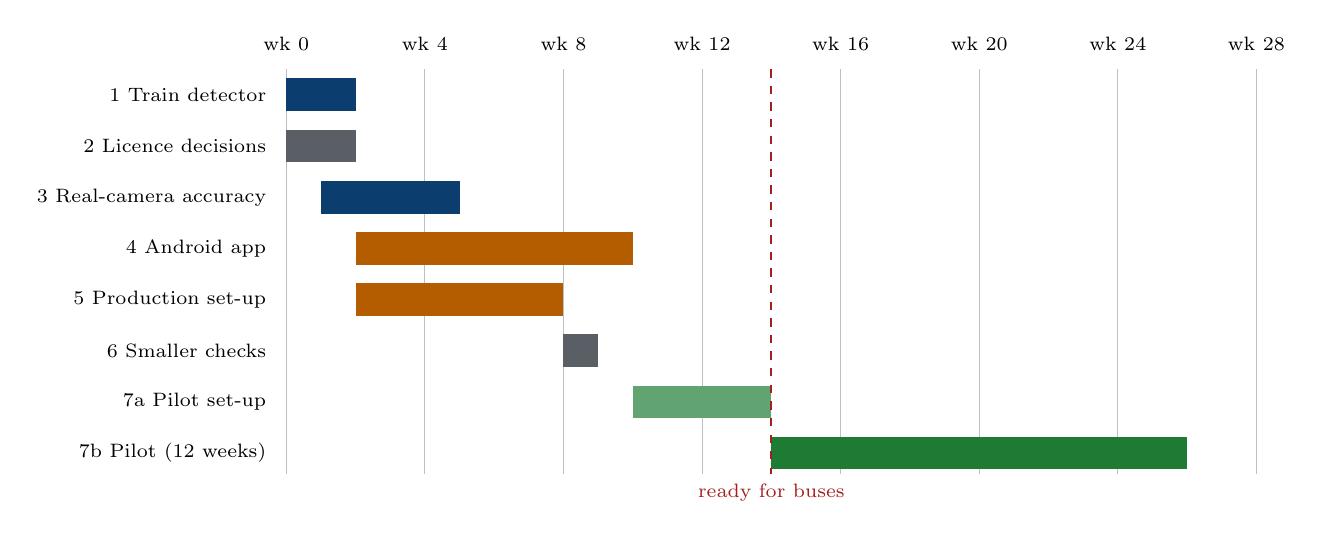
\begin{tikzpicture}[x=4.4mm, y=6.5mm]
  % weeks axis (0..28)
  \foreach \w in {0,4,...,28}{ \draw[gmgrey!40] (\w,0.5)--(\w,-7.4); \node[font=\scriptsize] at (\w,1) {wk \w}; }
  \gbar{0}{2}{0}{1 Train detector}{gmblue}
  \gbar{0}{2}{1}{2 Licence decisions}{gmgrey}
  \gbar{1}{5}{2}{3 Real-camera accuracy}{gmblue}
  \gbar{2}{10}{3}{4 Android app}{gmwarn}
  \gbar{2}{8}{4}{5 Production set-up}{gmwarn}
  \gbar{8}{9}{5}{6 Smaller checks}{gmgrey}
  \gbar{10}{14}{6}{7a Pilot set-up}{gmok!70}
  \gbar{14}{26}{7}{7b Pilot (12 weeks)}{gmok}
  \draw[gmbad, thick, dashed] (14,0.5)--(14,-7.4) node[below, font=\scriptsize, text=gmbad] {ready for buses};
\end{tikzpicture}
\caption{Indicative timeline (estimate). Software is ready now; about 14 weeks to a bus-ready system; a validated pilot
at about 26 weeks (6 months).}
\end{figure}

% ================================================================================================ 9
\section{How to run it}\label{sec:run}

On the Windows development laptop, from \code{C:\textbackslash gunthameter} in PowerShell (Linux/WSL: \code{make
<target>}):

\begin{center}
\begin{tabularx}{\textwidth}{@{}l X@{}}
\toprule
\textbf{Command} & \textbf{What it does}\\
\midrule
\code{.\textbackslash scripts\textbackslash windows\textbackslash tasks.ps1 test} & all CPU tests (276, about 5--6 minutes)\\
\code{tasks.ps1 measure-demo} & depth and volume on real Indian road images; no services needed\\
\code{tasks.ps1 seed} & build the demo database (OSM roads, GTFS, admin units, contracts, users)\\
\code{tasks.ps1 demo} & the full end-to-end demo (API on port 8000, web on port 5173)\\
\code{tasks.ps1 train} / \code{train-resume} & WP3 training in resumable 8-hour sessions\\
\code{tasks.ps1 report} & regenerate \code{reports/REPORT.md}\\
\bottomrule
\end{tabularx}
\end{center}
Demo logins (password \code{demo1234}): \code{admin}, \code{zonal\_khairatabad}, \code{engineer1},
\code{contractor1}, \code{contractor2}, \code{citizen1}.

% ================================================================================================ A
\appendix
\section{Key documents}
\begin{tabularx}{\textwidth}{@{}l X@{}}
\toprule
\code{docs/PLAN.md} & the full design and the work packages\\
\code{docs/DECISIONS.md} & deviations from the plan and the status of each build wave\\
\code{docs/HANDOFF.md} & where work stopped and the next steps\\
\code{docs/CONTRACTS.md} & frozen interfaces, state machines, API list\\
\code{docs/DEPTH\_METHOD.md} & the measurement method and its validation\\
\code{docs/CALIBRATION\_SOP.md} & depot calibration procedure (Telugu and English)\\
\code{docs/DEPLOYMENT\_TSRTC.md} & 20-bus pilot plan: hardware, power, heat, connectivity, server, schedule\\
\code{docs/LICENCES.md} & dataset, model and software licences, and the open decisions\\
\code{docs/DEMO\_SCRIPT.md} & 7-minute jury walkthrough\\
\code{edge/protocol.md} & how a bus device talks to the server\\
\code{reports/REPORT.md} & generated validation report\\
\bottomrule
\end{tabularx}

\section{Glossary}
\begin{tabularx}{\textwidth}{@{}l X@{}}
\toprule
$\sigma$ & standard uncertainty of a measurement; the truth lies within $\pm2\sigma$ about 95\,\% of the time\\
$d_{p95}$ & 95th-percentile depth of the cavity, the design depth\\
IRC & Indian Roads Congress (standards IRC:82, IRC:116, IRC:SP:100)\\
CRMP & Comprehensive Road Maintenance Programme (GHMC road packages with a contractor and liability period)\\
DLP & defect-liability period: time in which the contractor must fix failures of their work for free\\
SLA & service-level agreement: the deadline for a repair after a work order is issued\\
WO & work order\\
MB & Measurement Book (the record used for billing)\\
GTFS & General Transit Feed Specification (bus routes and schedules)\\
OSM & OpenStreetMap\\
AE / DEE / EE & Assistant / Deputy Executive / Executive Engineer\\
mAP50 & mean average precision at 50\,\% box overlap (detector accuracy)\\
PWA & progressive web app (installable, works offline)\\
\bottomrule
\end{tabularx}

\end{document}
